\documentclass[tikz,border=8pt]{standalone}
% Shared look for every TikZ diagram. Load with \input{../../tools/tikz-style.tex}
\usepackage[T1]{fontenc}
\usepackage{lmodern}
\renewcommand{\sfdefault}{lmr}  % diagrams use the same serif as the text
\usetikzlibrary{arrows.meta, positioning, shapes.geometric, calc, fit, backgrounds}
\definecolor{cblue}{HTML}{4C78A8}
\definecolor{corange}{HTML}{F58518}
\definecolor{cgreen}{HTML}{54A24B}
\definecolor{cred}{HTML}{E45756}
\definecolor{cpurple}{HTML}{B279A2}
\definecolor{cgrey}{HTML}{6B6B6B}
\tikzset{
  every picture/.style={font=\sffamily, line width=1.2pt},
  box/.style={draw=#1, fill=#1!12, rounded corners=4pt, align=center, inner sep=7pt, minimum height=1.1cm},
  box/.default=cgrey,
  arrow/.style={-{Stealth[length=3mm]}, draw=cgrey, line width=1.4pt},
  title/.style={font=\sffamily\bfseries\Large},
  note/.style={font=\sffamily\small, text=cgrey, align=center},
}
\AtBeginDocument{\hyphenpenalty=10000 \exhyphenpenalty=10000}

\begin{document}
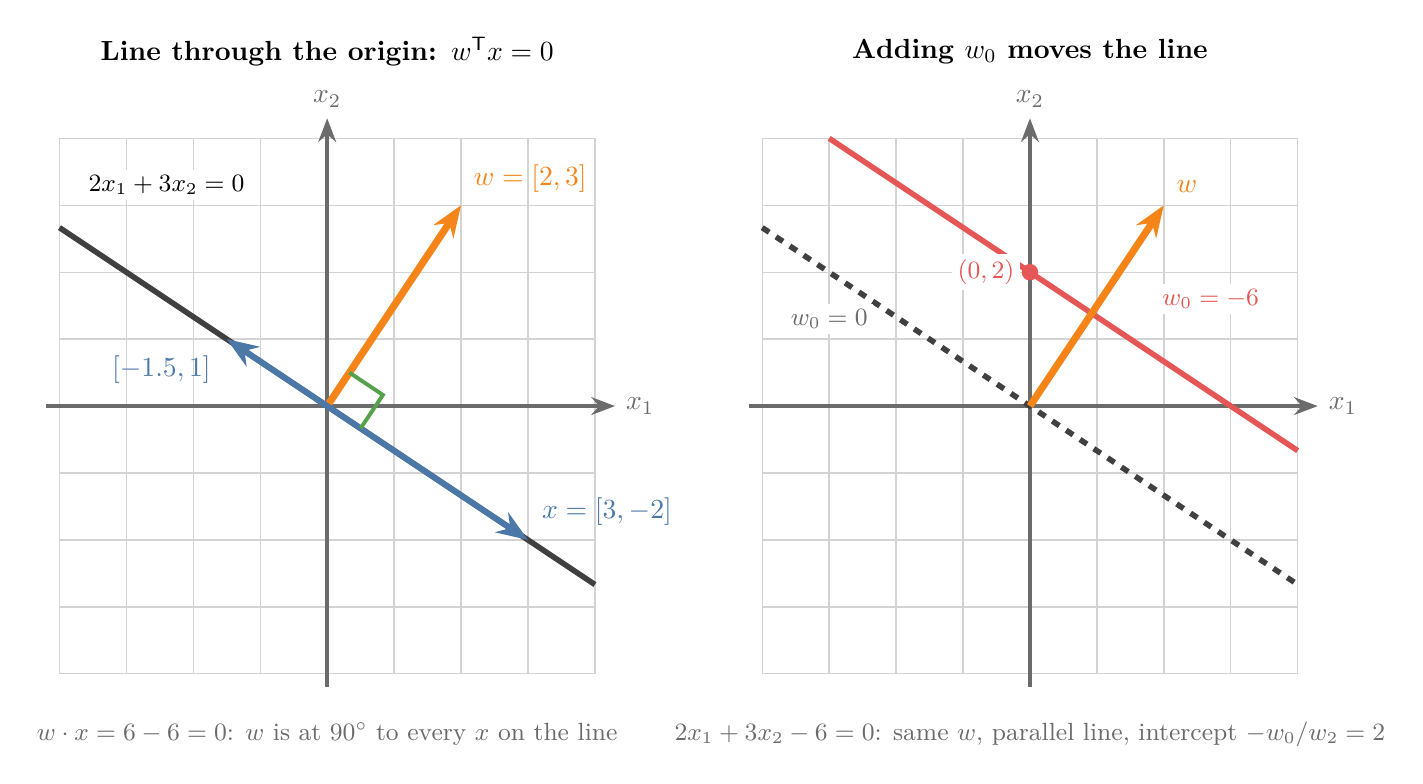
\begin{tikzpicture}[scale=0.85]
  \begin{scope}
    \node[font=\bfseries] at (0,5.3) {Line through the origin: $w^{\mathsf T}x = 0$};
    \draw[cgrey!30, line width=0.5pt] (-4,-4) grid (4,4);
    \draw[arrow, cgrey] (-4.2,0) -- (4.3,0) node[right] {$x_1$};
    \draw[arrow, cgrey] (0,-4.2) -- (0,4.3) node[above] {$x_2$};
    \draw[cgrey!60!black, line width=2pt] (-4,{8/3}) -- (4,{-8/3}); \node[font=\small, fill=white, inner sep=2pt] at (-2.4,3.3) {$2x_1 + 3x_2 = 0$};
    \draw[-{Stealth[length=4mm]}, corange, line width=2.6pt] (0,0) -- (2,3) node[above right, font=\bfseries] {$w = [2, 3]$};
    \draw[-{Stealth[length=4mm]}, cblue, line width=2.2pt] (0,0) -- (3,-2) node[above right=1pt, font=\bfseries] {$x = [3, -2]$};
    \draw[-{Stealth[length=4mm]}, cblue, line width=2.2pt] (0,0) -- (-1.5,1) node[below left=2pt, font=\bfseries] {$[-1.5, 1]$};
    \draw[cgreen, line width=1.4pt] (0.333,0.5) -- ++(0.5,-0.333) -- ++(-0.333,-0.5);
    \node[note] at (0,-4.9) {$w \cdot x = 6 - 6 = 0$: $w$ is at $90^\circ$ to every $x$ on the line};
  \end{scope}
  \begin{scope}[xshift=10.5cm]
    \node[font=\bfseries] at (0,5.3) {Adding $w_0$ moves the line};
    \draw[cgrey!30, line width=0.5pt] (-4,-4) grid (4,4);
    \draw[arrow, cgrey] (-4.2,0) -- (4.3,0) node[right] {$x_1$};
    \draw[arrow, cgrey] (0,-4.2) -- (0,4.3) node[above] {$x_2$};
    \draw[cgrey!60!black, line width=2pt, dashed] (-4,{8/3}) -- (4,{-8/3});
    \node[font=\small, text=cgrey, fill=white, inner sep=2pt] at (-3.0,1.3) {$w_0 = 0$};
    \draw[cred, line width=2pt] (-3,4) -- (4,{-2/3}) ; \node[font=\small, text=cred, fill=white, inner sep=2pt] at (2.7,1.6) {$w_0 = -6$};
    \fill[cred] (0,2) circle (3.5pt) node[left=3pt, font=\small, text=cred, fill=white, inner sep=2pt] {$(0, 2)$};
    \draw[-{Stealth[length=4mm]}, corange, line width=2.6pt] (0,0) -- (2,3) node[above right, font=\bfseries] {$w$};
    \node[note] at (0,-4.9) {$2x_1 + 3x_2 - 6 = 0$: same $w$, parallel line, intercept $-w_0/w_2 = 2$};
  \end{scope}
\end{tikzpicture}
\end{document}
